% =============================================================================
%  Section: Introduction
%  H1 Charged-Hadron SIDIS High-Q^2 Analysis Note
% =============================================================================
\section{Introduction}
\label{sec:introduction}

Semi-inclusive deep inelastic scattering (SIDIS) data provides the backbone for transverse-momentum-dependent (TMD) phenomenology. This note documents the H1 inclusive charged-hadron SIDIS analysis in the high-$\Qsq$ region.  The
measurement uses charged-particle tracks without particle identification.  The
reported charged-hadron categories are therefore only $\hplus$ and $\hminus$,
corrected to the summed primary-vertex yield of charged pions, kaons, and
protons.

The analysis uses the standard DIS and SIDIS kinematic variables.  With $k$ and
$k'$ denoting the incoming and scattered lepton four-momenta, $P$ the incoming
proton four-momentum, and $P_h$ the observed charged-hadron four-momentum, the
exchanged-photon four-momentum and inclusive DIS variables are
\begin{align}
  q &= k-k'\, , & \Qsq &= -q^2\, , \\
  x &= \frac{\Qsq}{2 P\cdot q}\, , &
  y &= \frac{P\cdot q}{P\cdot k}\, , \\
  W^2 &= (P+q)^2\, .
  \label{eq:intro:dis-variables}
\end{align}
The semi-inclusive variables used for the charged hadron are
\begin{align}
  z &= \frac{P\cdot P_h}{P\cdot q}\, , &
  \pTh &\equiv \left|\vec{P}_{h,T}\right|_{\gamma^{*}p\,\mathrm{c.m.}}\, .
  \label{eq:intro:sidis-variables}
\end{align}
Here $\pTh$ is the transverse momentum of the hadron with respect to the
virtual-photon direction in the $\gamma^{*}p$ center-of-mass frame.  The hadron
azimuth $\phih$ is defined around the virtual-photon axis in the same frame for
azimuthal diagnostic quantities.  In this measurement the photon four-momentum $q$ that
enters $z$, $\pTh$, and the $\gamma^{*}p$ frame is reconstructed with the
$e\Sigma$ method from the scattered electron and the hadronic final state, rather than
$q=k-k'$ from the electron alone, which amplifies electron-energy shifts at low $y$.
The $(\Qsq,x)$ cells and the $y$ cut use the $e\Sigma$ variables; the $E-p_z$ cut is unchanged.  The $x_F$ hemisphere cut keeps the
electron-like photon (Sec.~\ref{sec:selection:final-tracks}).

% The current high-$\Qsq$ working release covers $\Qsq>150~\GeVsq$ and uses a
% charge-separated four-dimensional grid in $(\Qsq,x,z,\pTh)$.  It contains 490
% published bins in total, 245 for $\hplus$ and 245 for $\hminus$.  The $z$ bin
% edges are $[0.0,0.05,0.1,0.2,0.3,0.5,0.7,1.0]$, with the first bin covering
% $0.0 \le z < 0.05$.

\begin{figure}[h!]
\centering
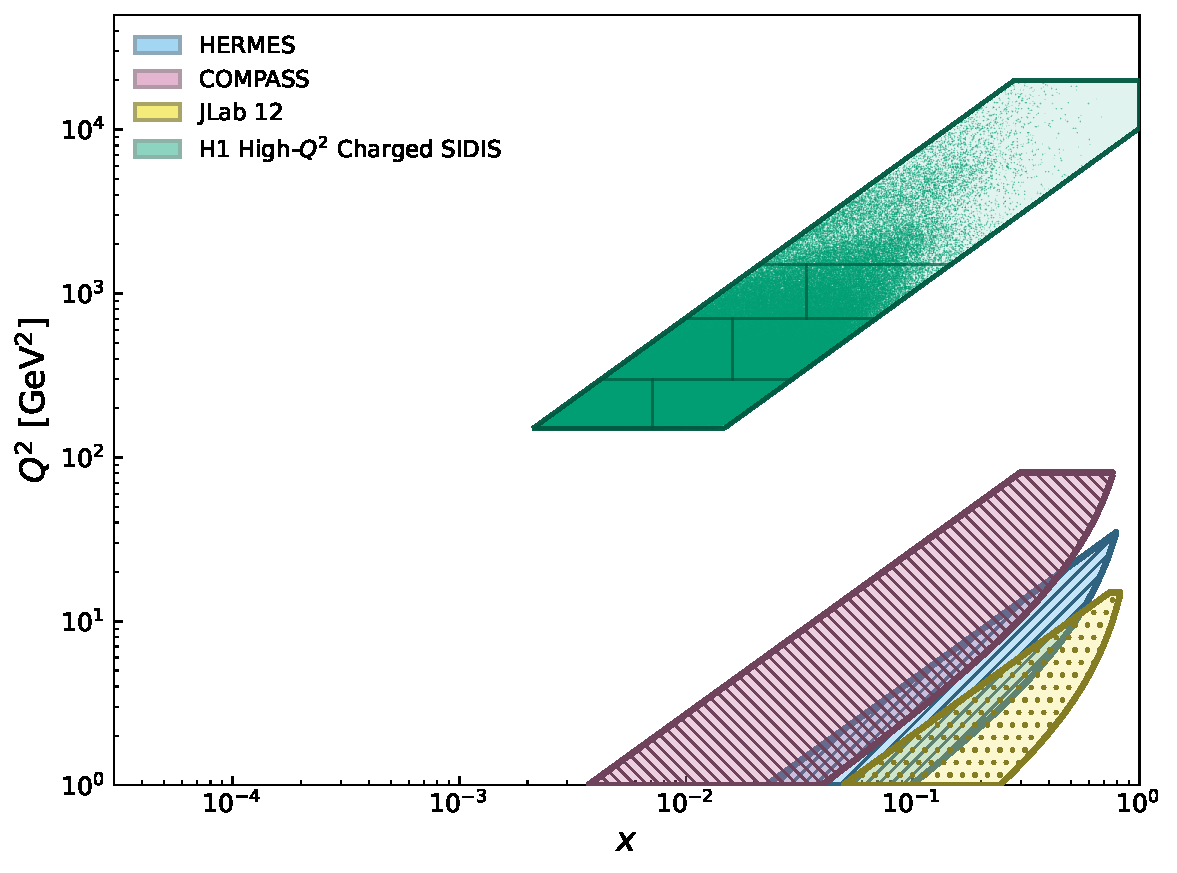
\includegraphics[width=0.82\textwidth]{figures/fig_kinematic_coverage_xQ2_H1.pdf}
\caption{H1 kinematic coverage in the $(x,\Qsq)$ plane.  The high-$\Qsq$
charged-hadron SIDIS measurement documented in this note uses the
$\Qsq>150~\GeVsq$ region and is binned further in $z$, $\pTh$, and charge.}
\label{fig:intro:kinematic-coverage-xq2}
\end{figure}

The radiative correction is applied to all cross sections in this note, which
are therefore Born-level.  A final publication-level review of the correction
is still pending, and the correction is not yet applied at the multiplicity
level.  The measurement is reported at the electron--proton cross-section
level; no virtual-photon--proton conversion is applied or required.
